\documentclass{beamer}
\mode<presentation>
\usetheme{CambridgeUS}
\usepackage[russian]{babel}
\usepackage[utf8]{inputenc}
\usepackage[T2A]{fontenc}
\usepackage{sansmathaccent}

\usepackage{verbatim}
\usepackage{alltt}

\pdfmapfile{+sansmathaccent.map}
\title[Artifical Intelligence]{Генетические алгоритмы}
\author{Наумов Д.А., доц. каф. КТ}
\date[08.10.2019] {Экспертные системы и искусственный интеллект, 2019}

\begin{document}

%ТИТУЛЬНЫЙ СЛАЙД
\begin{frame}
  \titlepage
\end{frame}
  
%СОДЕРЖАНИЕ ЛЕКЦИИ
\begin{frame}
  \frametitle{Содержание лекции}
  \tableofcontents  
\end{frame}

\section{Эволюционные вычисления}
\begin{frame}
\begin{block}{Эволюционные вычисления }
общий термин для описания алгоритмов поиска, оптимизации, машинного обучения или анализа данных, основанных на некоторых формализованных принципах естественного эволюционного отбора и генетики.
\end{block}
Основные парадигмы:
\begin{itemize}
\item генетические алгоритмы – двоичное и вещественное представление решений-хромосом
\item генетическое программирование – программы, деревья графы как представления решений-хромосом
\item эволюционные стратегии – вещественные вектора или
скаляры как представления решений-хромосом
\item эволюционное программирование – конечный автомат как представления решений-хромосом
\end{itemize}
\end{frame}

\begin{frame}{Три основные принципа эволюционного подхода}
Charles Darwin, 1859. 

Принцип выживания сильнейших и естественный отбор
\begin{figure}[h]
\centering
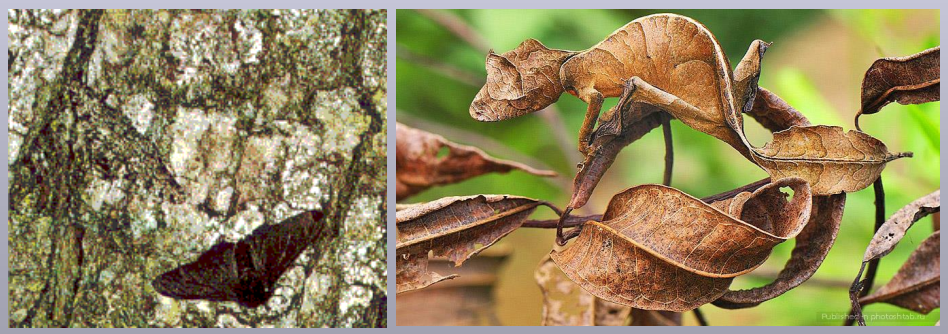
\includegraphics[scale=0.4]{images/lec04-pic01.png}
\end{figure}
\end{frame}

\begin{frame}{Три основные принципа эволюционного подхода}
Мендель, 1865. 

Основной принцип механизма наследования – хромосомы потомков состоят из частей хромосом их родителей
\begin{figure}[h]
\centering
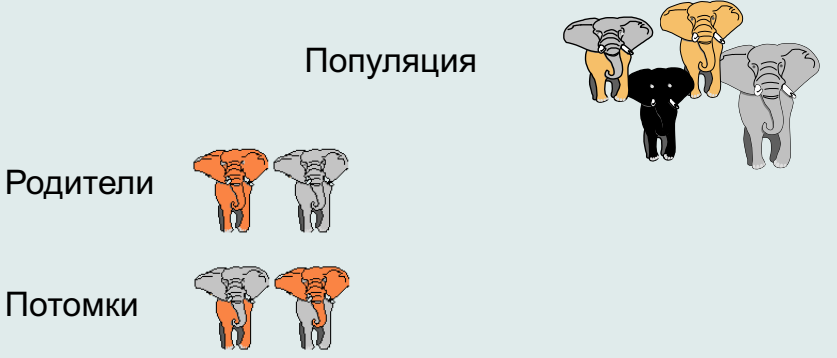
\includegraphics[scale=0.4]{images/lec04-pic02.png}
\end{figure}
\end{frame}

\begin{frame}{Три основные принципа эволюционного подхода}
де Вре, 1900

Принцип мутации – существенные (разные) изменения свойств потомков и приобретение ими свойств, отсутствующих у родителей
\begin{figure}[h]
\centering

\includegraphics[scale=0.4]{images/lec04-pic03.png}
\end{figure}
\end{frame}

\begin{frame}
\begin{block}{Генетические алгоритмы}
случайно направленные поисковые алгоритмы, которые эмулируют процесс естественной
эволюции для построения (суб)оптимального решения задачи.
\end{block}
\begin{itemize}
\item реализуют принцип <<выживание сильнейших>> среди рассматриваемых
структур;
\item формирует и изменяет поисковый алгоритм на основе моделирования эволюции
\end{itemize}
Некоторые основатели и исследователи: J.Holland, D.Goldberg, Z.Michalewicz 
\end{frame}

\begin{frame}{Генетические алгоритмы}
Генетический алгоритм характеризуется следующими основными параметрами:
\[ГА=P^0, \lambda, l, s, p, f, t\]
где
\begin{itemize}
\item $P^0 = (X^0_1...X^0_\lambda)$ - исходная популяция;
\item $X^0_1$ - решение задачи, представленное в виде хромосомы;
\item $\lambda$ - размер популяции
\item $l$ - длина каждой хромосомы;
\item $s$ - оператор отбора;
\item $p$ - отображение, определяющее рекомбинацию;
\item $f$ - целевая функция;
\item $t$ - критерий остановки алгоритма.
\end{itemize}
\end{frame}

\begin{frame}{Блок-схема классического генетического алгоритма}
\begin{figure}[h]
\centering
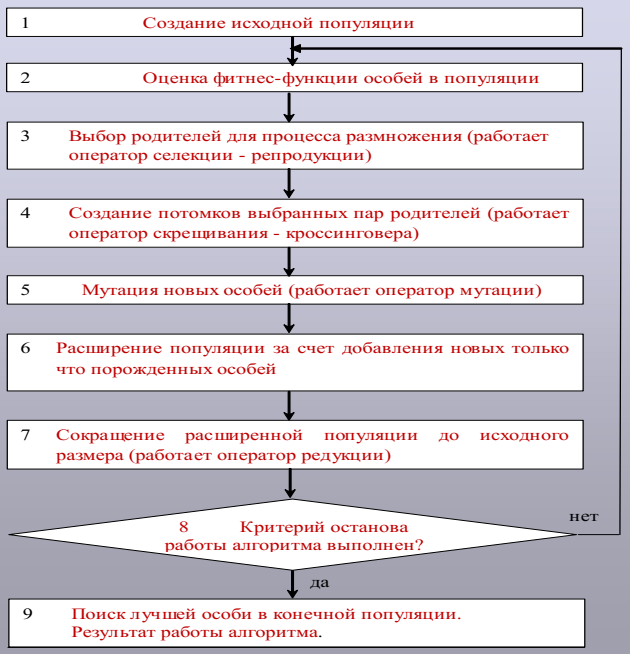
\includegraphics[scale=0.4]{images/lec04-pic04.png}
\end{figure}
\end{frame}

\begin{frame}{Кодирование хромосомы}
\begin{block}{Хромосома}
потенциальное решение представляется двоичной строкой – искусственной хромосомой, где каждый <<ген>> равен 0 или 1.
\end{block}
\begin{figure}[h]
\centering
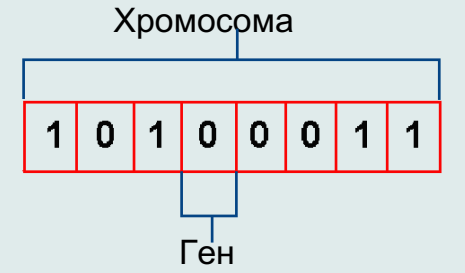
\includegraphics[scale=0.4]{images/lec04-pic05.png}
\end{figure}
\begin{block}{Популяция}
множество потенциальных решений. Развивается по законам искусственной эволюции
на основе генетических операторов
\end{block}
\end{frame}

\begin{frame}{Кодирование хромосомы}
\begin{figure}[h]
\centering
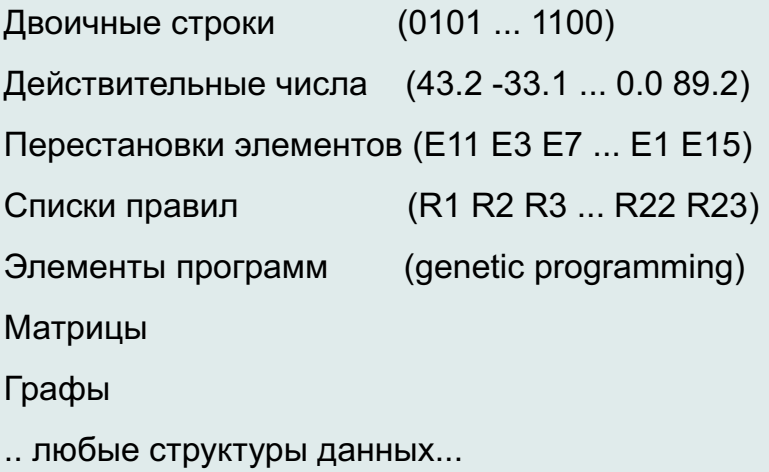
\includegraphics[scale=0.5]{images/lec04-pic06.png}
\end{figure}
\end{frame}

\begin{frame}{Оператор селекции}
\begin{block}{Ассиметричное колесо рулетки}
Популяция отображается на колесо рулетки, где каждая особь представляется сектором, размер которого пропорционален значению фитнесс функции.
\end{block}
\begin{figure}[h]
\centering
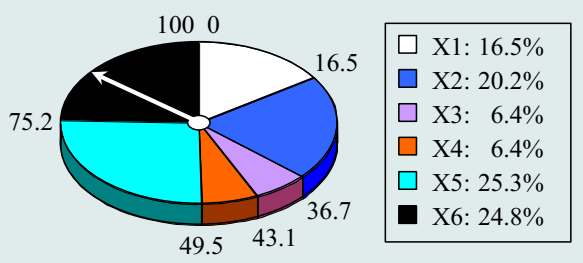
\includegraphics[scale=0.4]{images/lec04-pic07.png}
\end{figure}
Особи выбираются путем повторного вращения на основе стохастического выбора с возвращением.
\end{frame}

\begin{frame}{Оператор кроссинговера}
\begin{figure}[h]
\centering
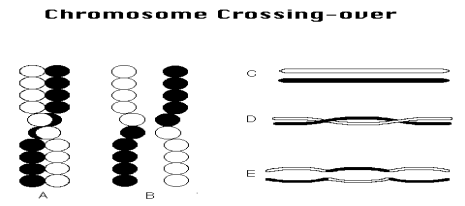
\includegraphics[scale=0.4]{images/lec04-pic08.png}
\end{figure}
Одноточечной или простой оператор кроссинговера в выполняется с вероятностью Pc в 2 этапа:
\begin{figure}[h]
\centering
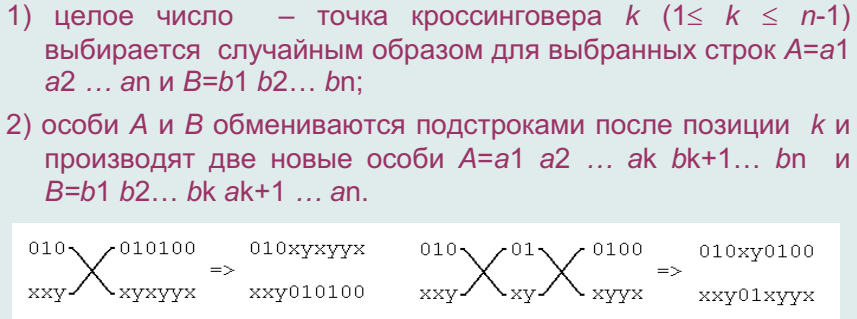
\includegraphics[scale=0.4]{images/lec04-pic09.png}
\end{figure}
\end{frame}

\begin{frame}{Оператор мутации}
Оператор мутации случайным образом (с малой вероятностью Pm) изменяет значения некоторых генов особей популяции: 

01001011 -> 01000011
\begin{figure}[h]
\centering
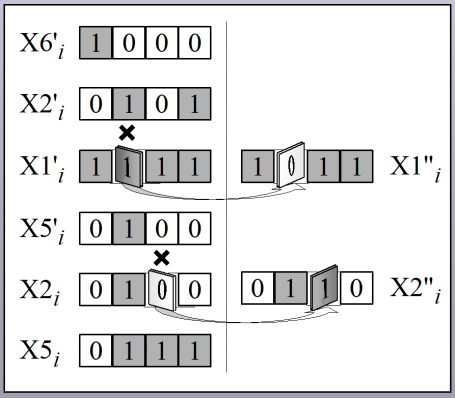
\includegraphics[scale=0.4]{images/lec04-pic10.png}
\end{figure}
\end{frame}

\begin{frame}{Пример}
Найти (для простоты) целочисленное значение х на отрезке от $[0,31]$,
при котором функция $f(x)=x^2$ принимает максимальное значение.
\begin{figure}[h]
\centering
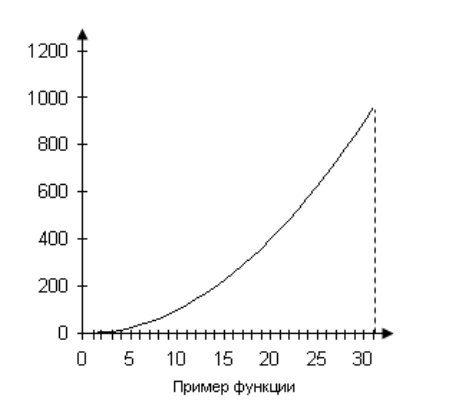
\includegraphics[scale=0.5]{images/lec04-pic11.png}
\end{figure}
\end{frame}

\begin{frame}
\begin{figure}[h]
\centering
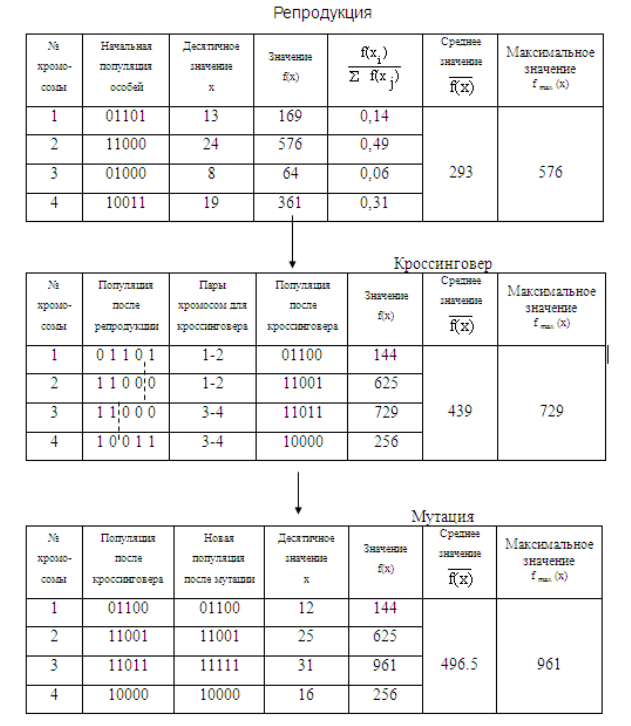
\includegraphics[scale=0.4]{images/lec04-pic12.png}
\end{figure}
\end{frame}

\begin{frame}
\begin{figure}[h]
\centering
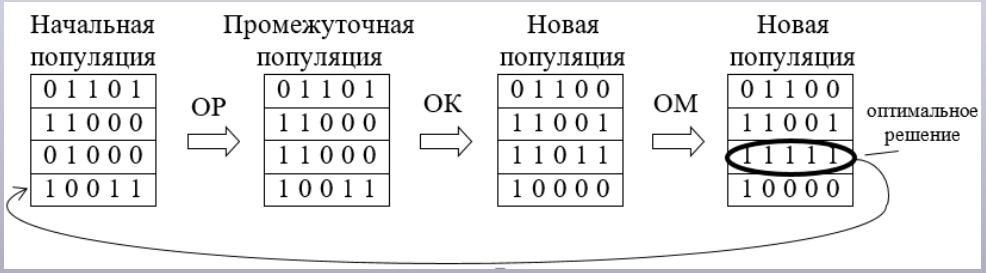
\includegraphics[scale=0.45]{images/lec04-pic13.png}
\end{figure}
\end{frame}

\begin{frame}{Пример}
Рассмотрим $f(x)=(1,85 -x)*cos(3,5x – 0,5)$, необходимо найти вещественное x, которое максимизирует f
\begin{figure}[h]
\centering
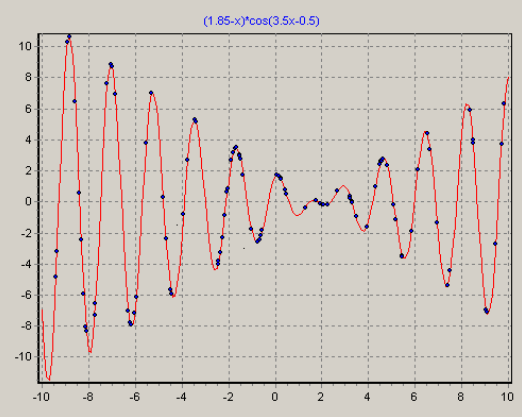
\includegraphics[scale=0.5]{images/lec04-pic14.png}
\end{figure}
Пример функции с популяцией особей в начале эволюции
\end{frame}

\begin{frame}{Кодирование решения}
\begin{itemize}
\item Для представления вещественного решения (хромосомы) будем также использовать двоичный вектор, который применяется в классическом простом ГА.
\item Его длина зависит от требуемой точности решения, которую
в данном случае положим 3 знака после запятой.
\item Поскольку отрезок области решения имеет длину 20, для
достижения заданной точности отрезок [a,c]= [-10,+10]
должен быть разбит на равные части (маленькие отрезки),
число которых должно быть не менее 20*1000.
\item В качестве двоичного представления используем двоичный
код номера (маленького) отрезка. Этот код позволяет
определить соответствующее ему вещественное число,
если известны границы области решения
\end{itemize}
\end{frame}

\begin{frame}{Кодирование решения}
Отображение из двоичного представления в вещественное число из отрезка: 
\begin{figure}[h]
\centering
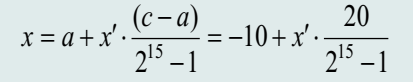
\includegraphics[scale=0.75]{images/lec04-pic15.png}
\end{figure}
Хромосомы (000000000000000) и (111111111111111) представляют границы отрезка –10 и +10 соответственно.
\end{frame}

\begin{frame}{Работа ГА}
\begin{figure}[h]
\centering
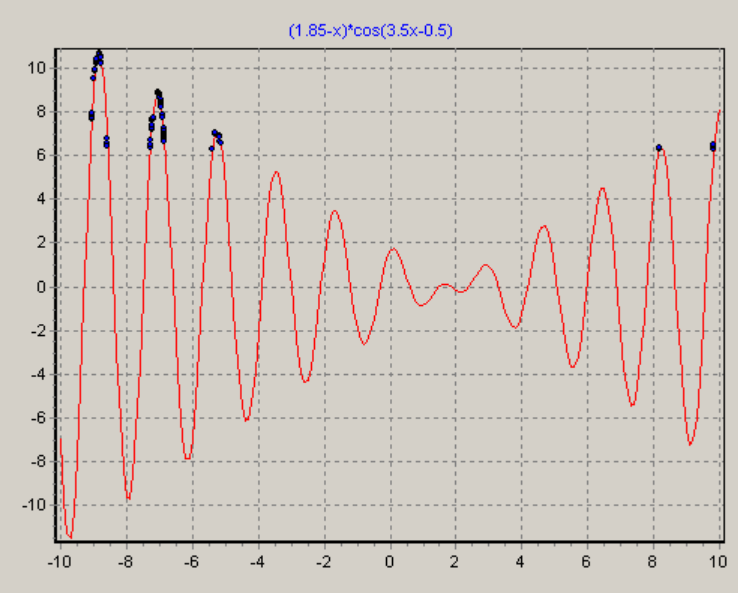
\includegraphics[scale=0.4]{images/lec04-pic16.png}
\end{figure}
\end{frame}

\begin{frame}{Работа ГА}
\begin{figure}[h]
\centering
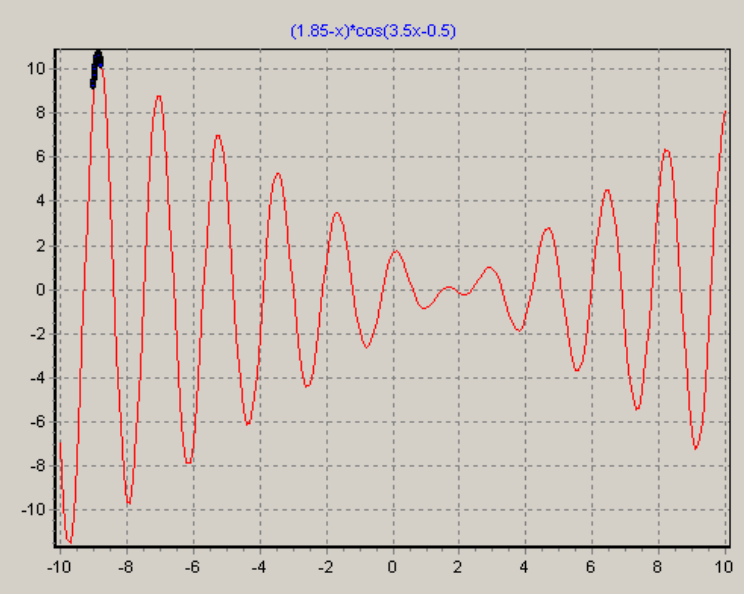
\includegraphics[scale=0.4]{images/lec04-pic17.png}
\end{figure}
\end{frame}

\begin{frame}{Пример оптимизации функции двух переменных}
\begin{figure}[h]
\centering
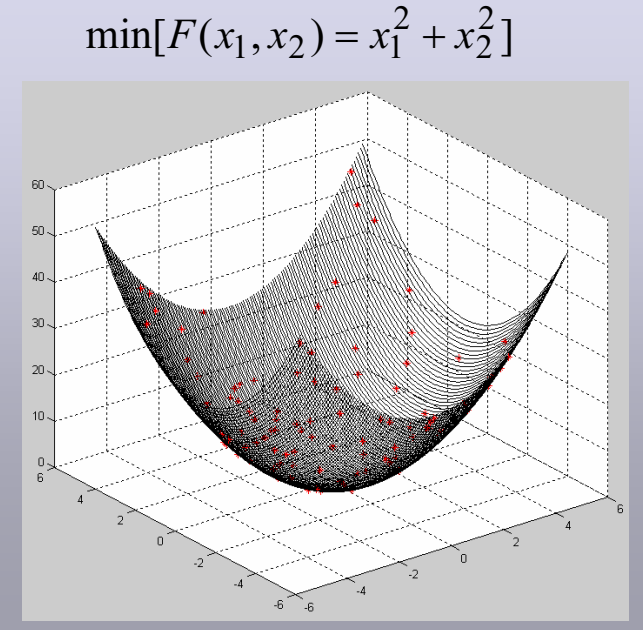
\includegraphics[scale=0.4]{images/lec04-pic18.png}
\end{figure}
\end{frame}

\begin{frame}{Пример оптимизации функции двух переменных}
\begin{figure}[h]
\centering
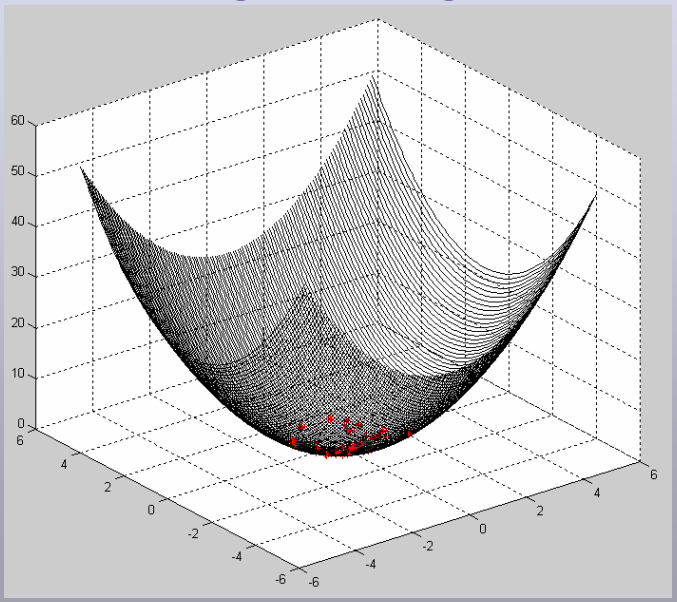
\includegraphics[scale=0.4]{images/lec04-pic19.png}
\end{figure}
\end{frame}

\begin{frame}{Пример оптимизации функции двух переменных}
\begin{figure}[h]
\centering
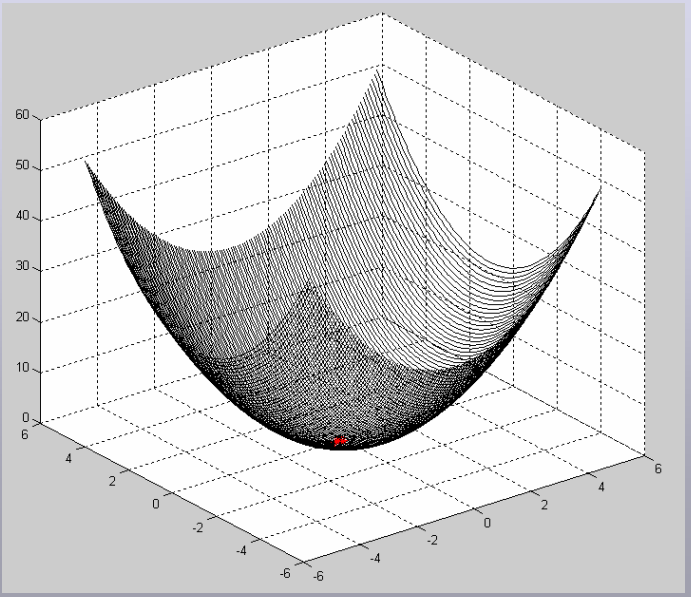
\includegraphics[scale=0.4]{images/lec04-pic20.png}
\end{figure}
\end{frame}

\begin{frame}{Оператор селекции: рулетка}
\begin{figure}[h]
\centering
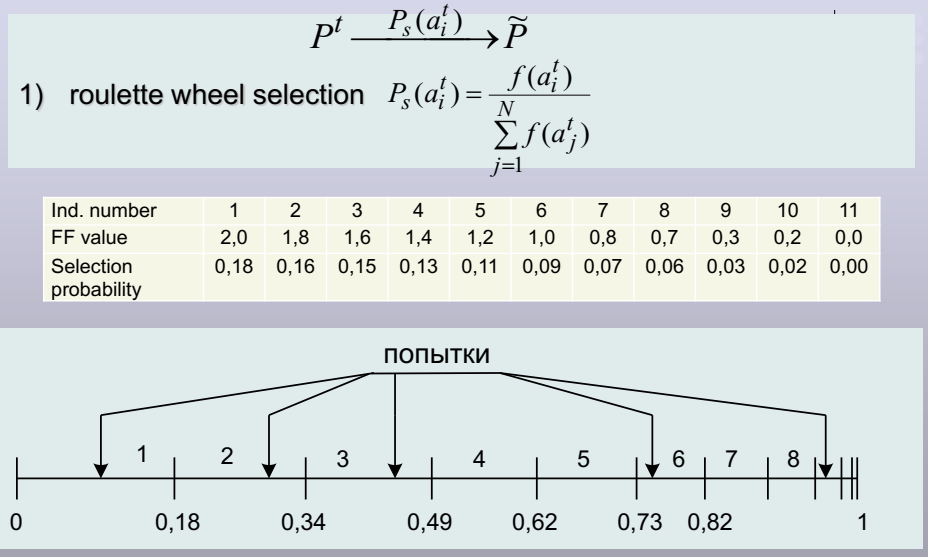
\includegraphics[scale=0.4]{images/lec04-pic21.png}
\end{figure}
\end{frame}

\begin{frame}{Оператор селекции: линейный ранк}
\begin{figure}[h]
\centering
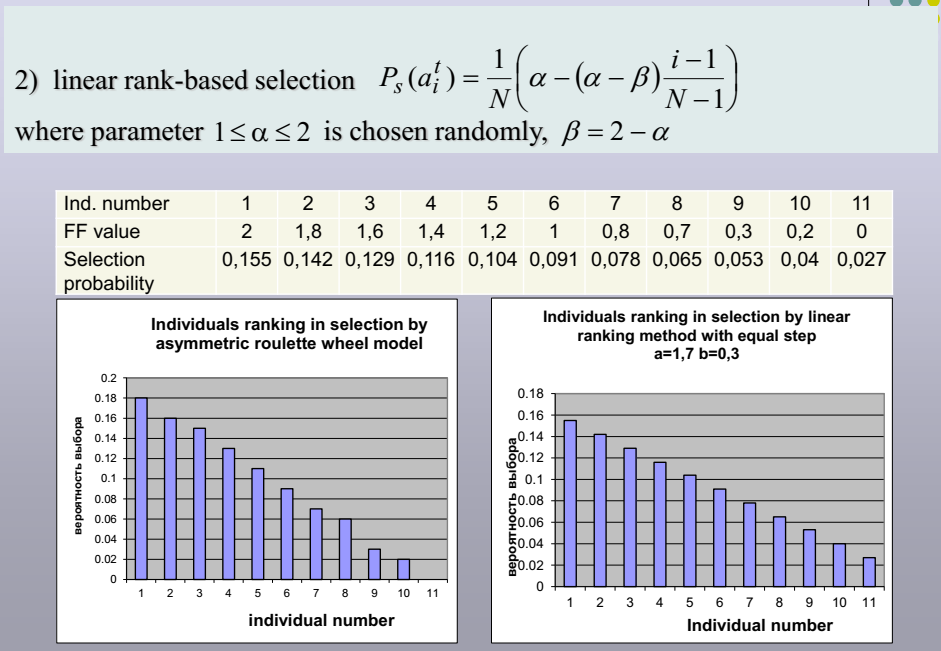
\includegraphics[scale=0.4]{images/lec04-pic22.png}
\end{figure}
\end{frame}

\begin{frame}{Оператор селекции: турнирный отбор}
\begin{figure}[h]
\centering
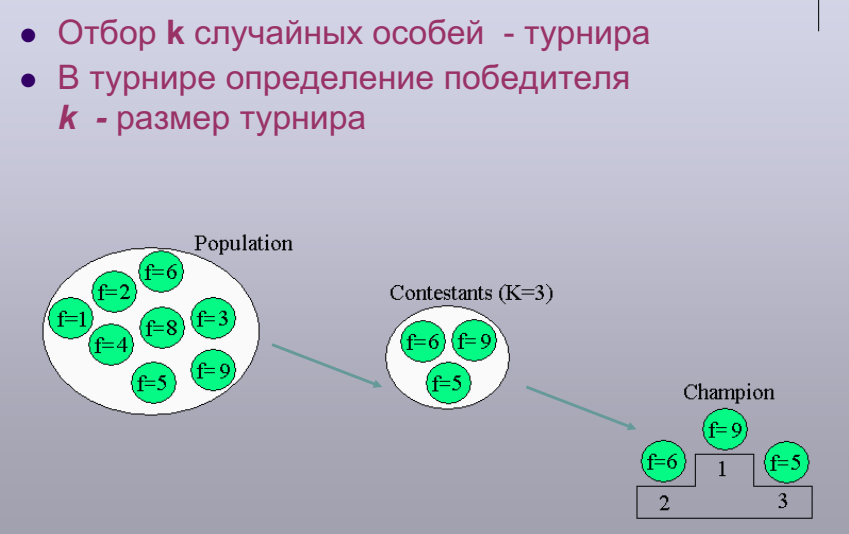
\includegraphics[scale=0.4]{images/lec04-pic23.png}
\end{figure}
\end{frame}

\begin{frame}{Пример: дискретная рекомбинация}
\begin{figure}[h]
\centering
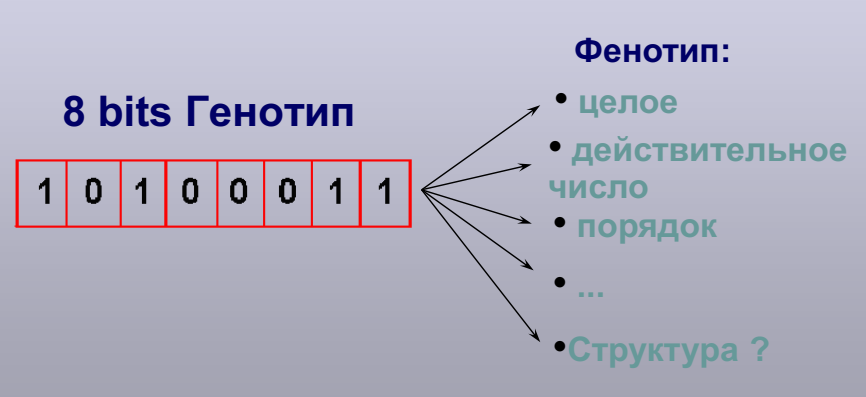
\includegraphics[scale=0.4]{images/lec04-pic24.png}
\end{figure}
\end{frame}

\begin{frame}{Пример: дискретная рекомбинация}
Двоичный алфавит:
\begin{figure}[h]
\centering
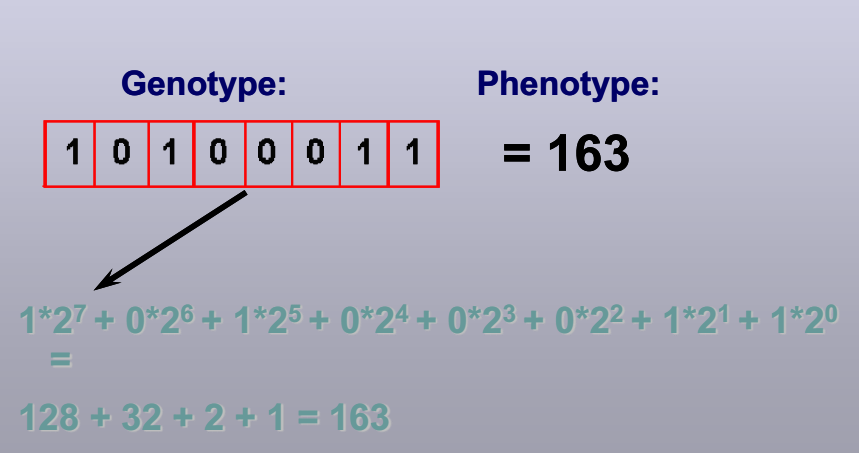
\includegraphics[scale=0.4]{images/lec04-pic25.png}
\end{figure}
\end{frame}

\begin{frame}{Пример: дискретная рекомбинация}
Действительное число:
\begin{figure}[h]
\centering
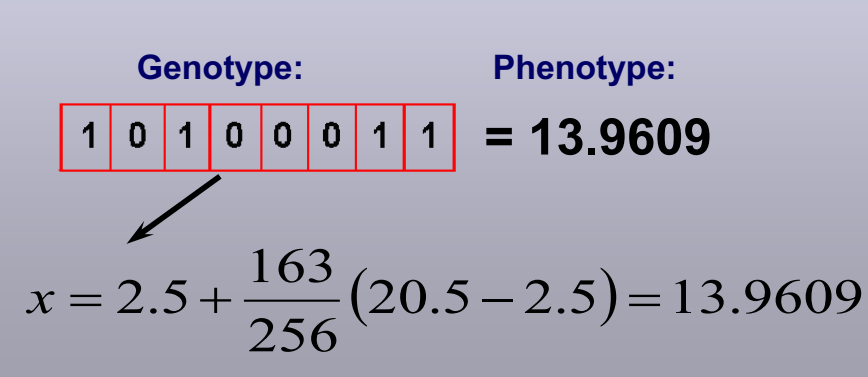
\includegraphics[scale=0.4]{images/lec04-pic26.png}
\end{figure}
\end{frame}

\begin{frame}{Пример: дискретная рекомбинация}
Фенотип как очередь:
\begin{figure}[h]
\centering
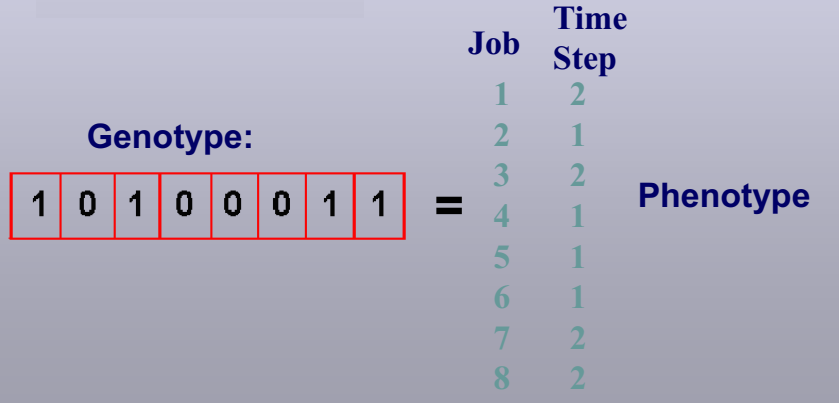
\includegraphics[scale=0.4]{images/lec04-pic27.png}
\end{figure}
\end{frame}

\begin{frame}{Пример: дискретная рекомбинация}
Действительное представление в ввиде массива чисел:
\begin{figure}[h]
\centering
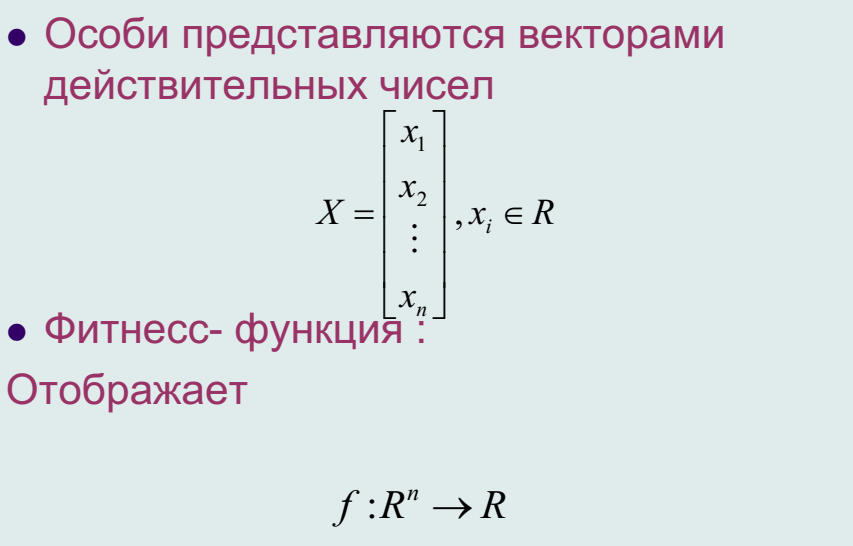
\includegraphics[scale=0.4]{images/lec04-pic28.png}
\end{figure}
\end{frame}

\begin{frame}{Пример: дискретная рекомбинация}
Древовидное представление:
\begin{figure}[h]
\centering
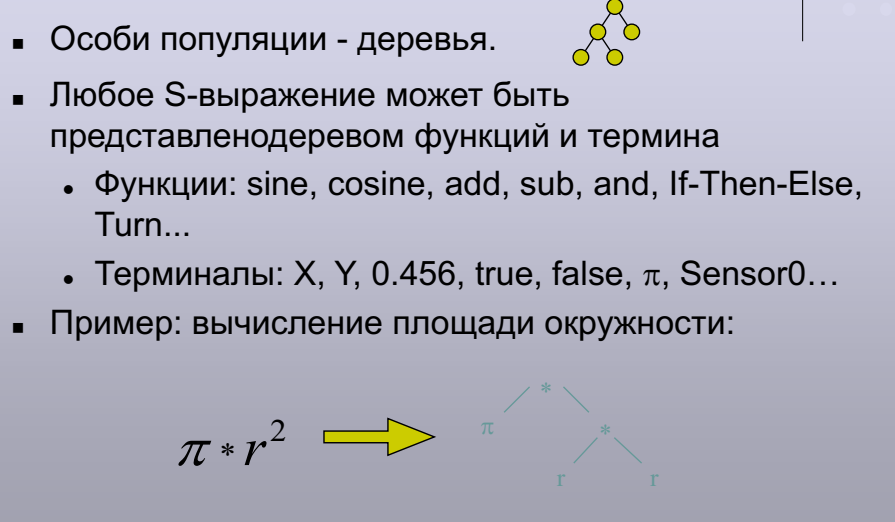
\includegraphics[scale=0.4]{images/lec04-pic29.png}
\end{figure}
\end{frame}

\begin{frame}{Оператор мутации}
\begin{itemize}
\item Операторы мутации должны позволять исследовать пространство решений
\item Важен размер шага мутации, желательно его контролировать
\item Мутация должна производить правильные решения
\end{itemize}
\begin{figure}[h]
\centering
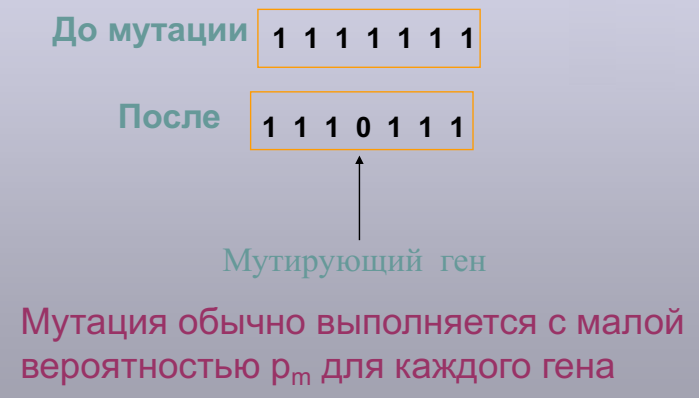
\includegraphics[scale=0.4]{images/lec04-pic30.png}
\end{figure}
\end{frame}

\begin{frame}
Мутация для действительного представления
\begin{itemize}
\item Выполняется путем наложения случайного шума
\item Часто используется Гауссово, нормальное распределение $x'_i=x_i+N(0, \sigma)$
\end{itemize}
Мутация для упорядоченного представления (случайный выбор генов и обмен)
\begin{figure}[h]
\centering
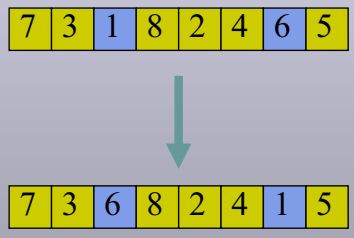
\includegraphics[scale=0.4]{images/lec04-pic31.png}
\end{figure}
\end{frame}

\begin{frame}{Операторы рекомбинации}
\begin{itemize}
\item Потомок должен взять что то от каждого родителя.
\item Оператор рекомбинации должен разрабатываться вместе с кодированием(представлением) решения.
\item Рекомбинация должна производить правильные решения.
\item Рекомбинация выполняется с вероятностью $P_c$.
\end{itemize}
\end{frame}

\begin{frame}
\begin{figure}[h]
\centering
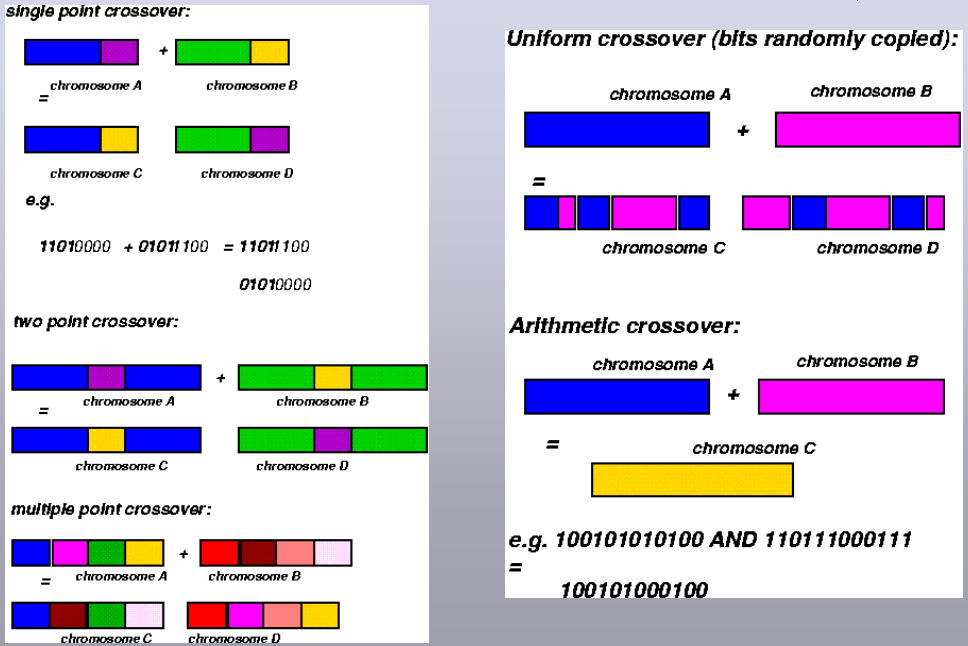
\includegraphics[scale=0.4]{images/lec04-pic32.png}
\end{figure}
\end{frame}

\begin{frame}{Однородный кроссинговер}
Производит потомка от 2-х заданных родителей следующим образом
\begin{figure}[h]
\centering
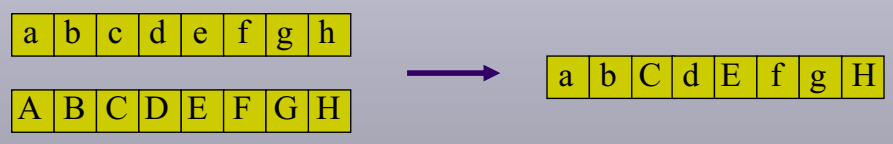
\includegraphics[scale=0.4]{images/lec04-pic33.png}
\end{figure}
\end{frame}

\begin{frame}{Арифметический кроссинговер}
По 2-м данным родителям потомок производится следующим образом
\begin{figure}[h]
\centering
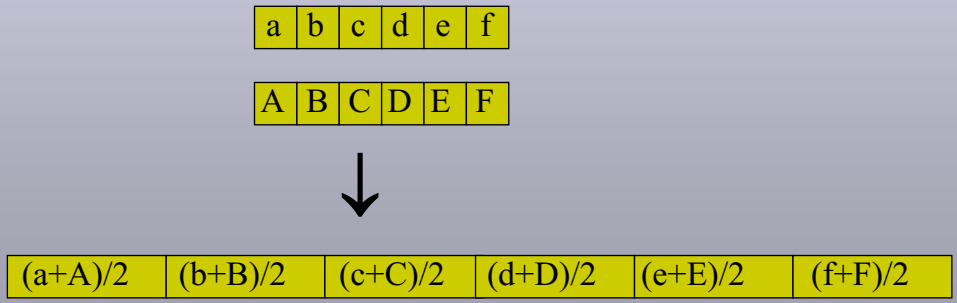
\includegraphics[scale=0.4]{images/lec04-pic34.png}
\end{figure}
\end{frame}

\begin{frame}{Рекомбинация для упорядоченного представления}
По 2-м данным родителям потомок производится следующим образом
\begin{figure}[h]
\centering
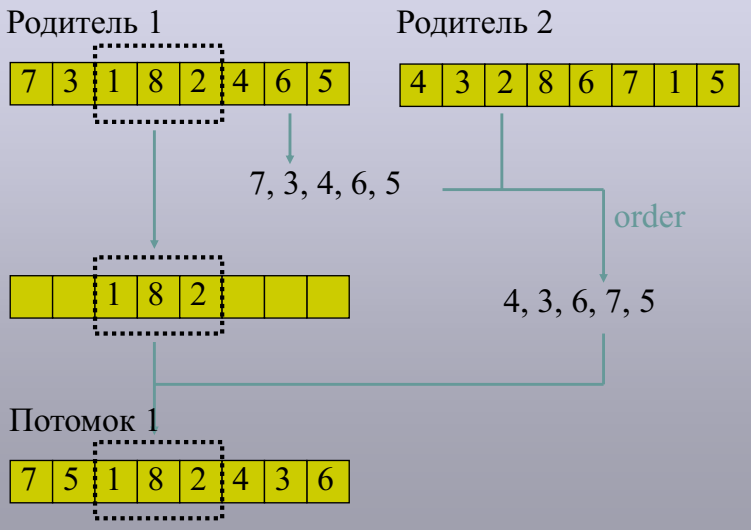
\includegraphics[scale=0.4]{images/lec04-pic35.png}
\end{figure}
\end{frame}

\begin{frame}{Задача коммивояжера}
Коммивояжер (бродячий торговец) должен выйти из первого города,
посетить по одному разу в некотором порядке все города и вернуться в
исходный город. Расстояния между городами известны. В каком порядке следует обходить города, чтобы замкнутый путь (тур) коммивояжера был кратчайшим?
\begin{figure}[h]
\centering

\includegraphics[scale=0.4]{images/lec04-pic36.png}
\end{figure}
\end{frame}

\begin{frame}{Задача коммивояжера: формальная постановка}
\begin{itemize}
\item имеется полный взвешенный ориентированный граф без петель G с множеством вершин N={1,2,…,n};
\item веса всех дуг неотрицательны;
\item в этом графе требуется найти гамильтонов цикл с минимальной стоимостью.
\item Исходная информация по ЗК представляется в виде
матрицы - вес дуги (i,j) графа G все элементы главной
диагонали нулевые (но в некоторых постановках полагаются).
\item Тур коммивояжера может быть описан циклической
перестановкой t=(j1,j2,..,jn,j1), причём все j1..jn – разные;
повторяющийся в начале и в конце номер города j1,
показывает, что перестановка циклическая.
\item Пространством поиска решений этой задачи является множество перестановок n городов.
\item Размерность пространства поиска задачи пропорциональна (n-1)!
\end{itemize}
\end{frame}

\begin{frame}{Задача коммивояжера}
\begin{figure}[h]
\centering
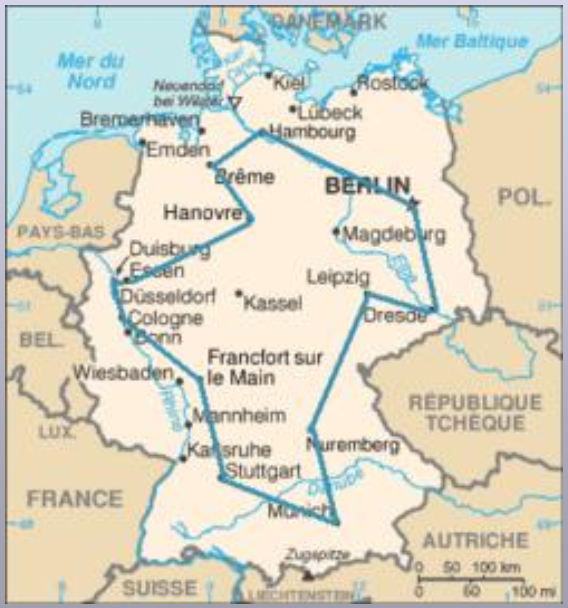
\includegraphics[scale=0.4]{images/lec04-pic37.png}
\end{figure}
\end{frame}

\begin{frame}{Представление решения}
\begin{figure}[h]
\centering
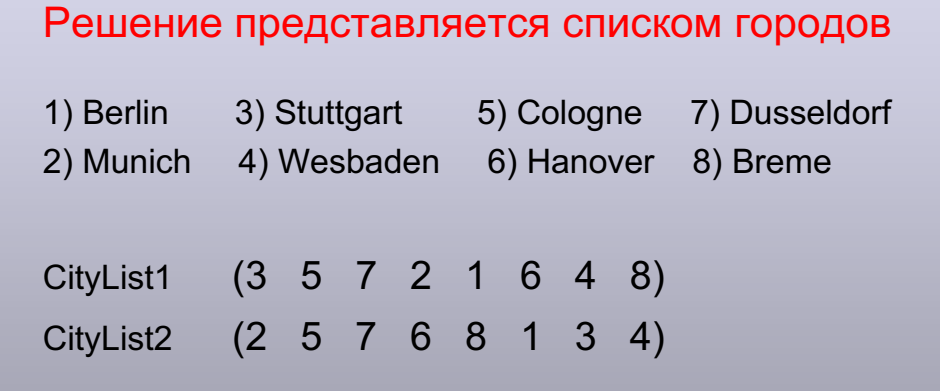
\includegraphics[scale=0.4]{images/lec04-pic38.png}
\end{figure}
\end{frame}

\begin{frame}{Мутация}
\begin{figure}[h]
\centering
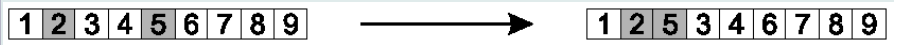
\includegraphics[scale=0.4]{images/lec04-pic39.png}
\end{figure}
\end{frame}

\begin{frame}{Кроссинговер}
\begin{figure}[h]
\centering
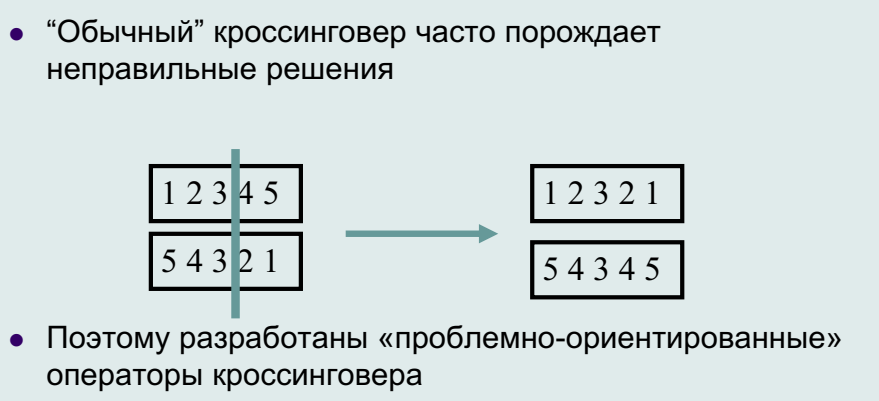
\includegraphics[scale=0.4]{images/lec04-pic40.png}
\end{figure}
\end{frame}

\begin{frame}{Упорядоченный кроссинговер}
\begin{figure}[h]
\centering
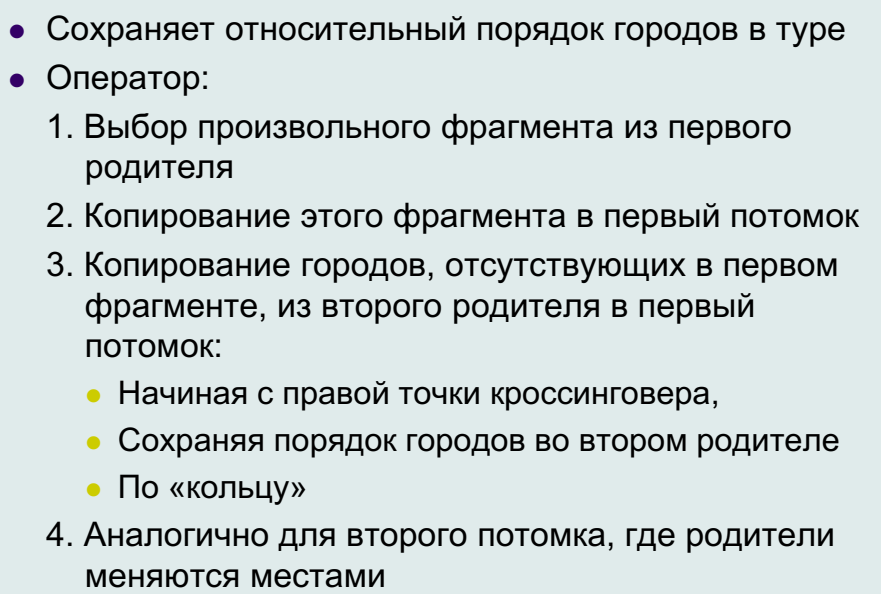
\includegraphics[scale=0.4]{images/lec04-pic41.png}
\end{figure}
\end{frame}

\begin{frame}{Пример упорядоченного кроссинговера}
\begin{figure}[h]
\centering
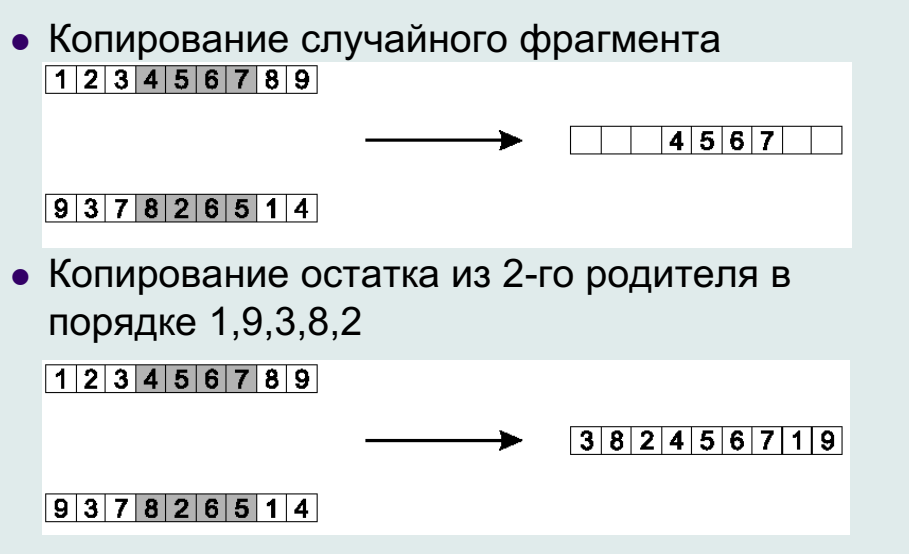
\includegraphics[scale=0.4]{images/lec04-pic42.png}
\end{figure}
\end{frame}

\begin{frame}{ЗК: 30 городов}
\begin{figure}[h]
\centering
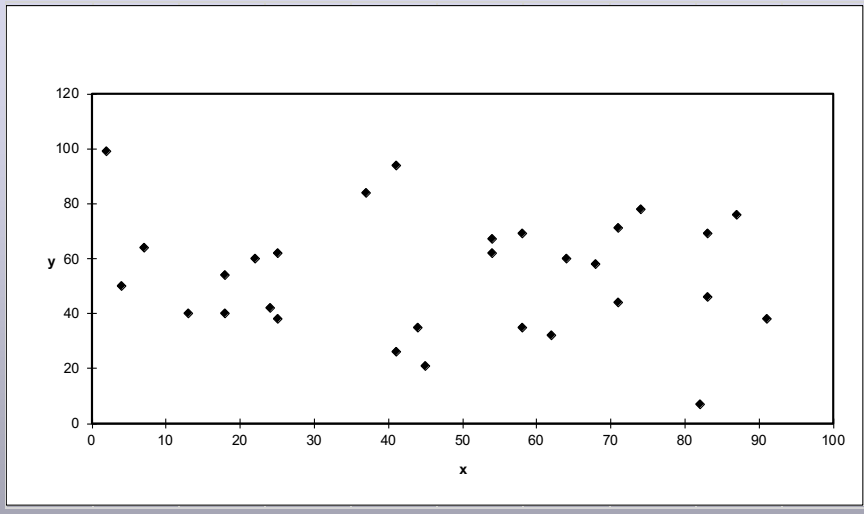
\includegraphics[scale=0.4]{images/lec04-pic43.png}
\end{figure}
\end{frame}

\begin{frame}{ЗК: 30 городов}
\begin{figure}[h]
\centering
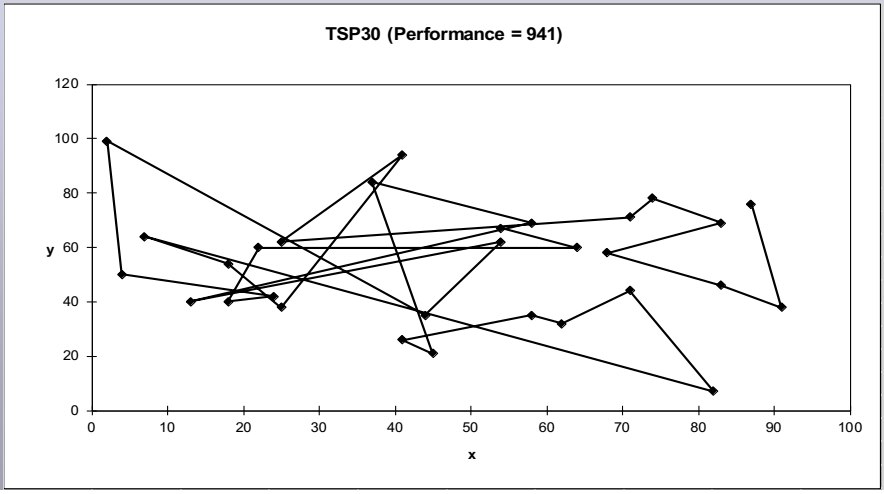
\includegraphics[scale=0.4]{images/lec04-pic44.png}
\end{figure}
\end{frame}

\begin{frame}{ЗК: 30 городов}
\begin{figure}[h]
\centering
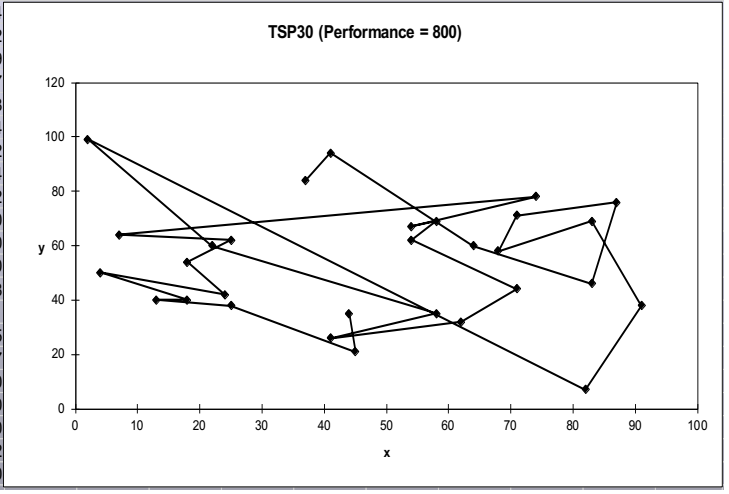
\includegraphics[scale=0.4]{images/lec04-pic45.png}
\end{figure}
\end{frame}

\begin{frame}{ЗК: 30 городов}
\begin{figure}[h]
\centering
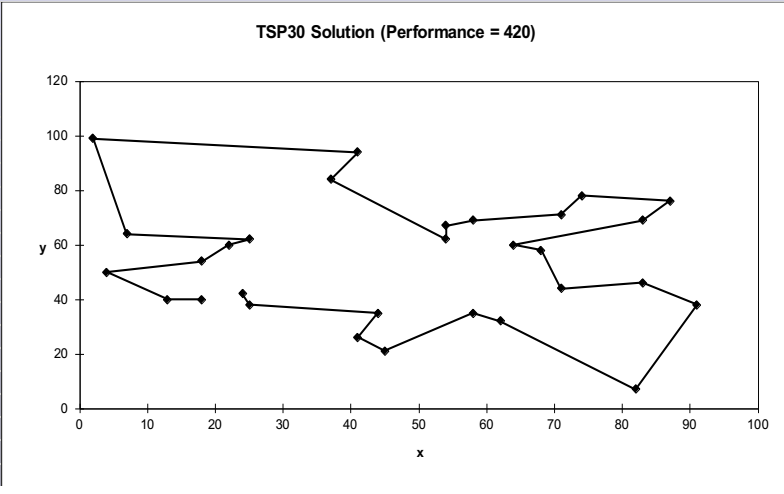
\includegraphics[scale=0.4]{images/lec04-pic46.png}
\end{figure}
\end{frame}

\begin{frame}{ЗК: 30 городов}
\begin{figure}[h]
\centering
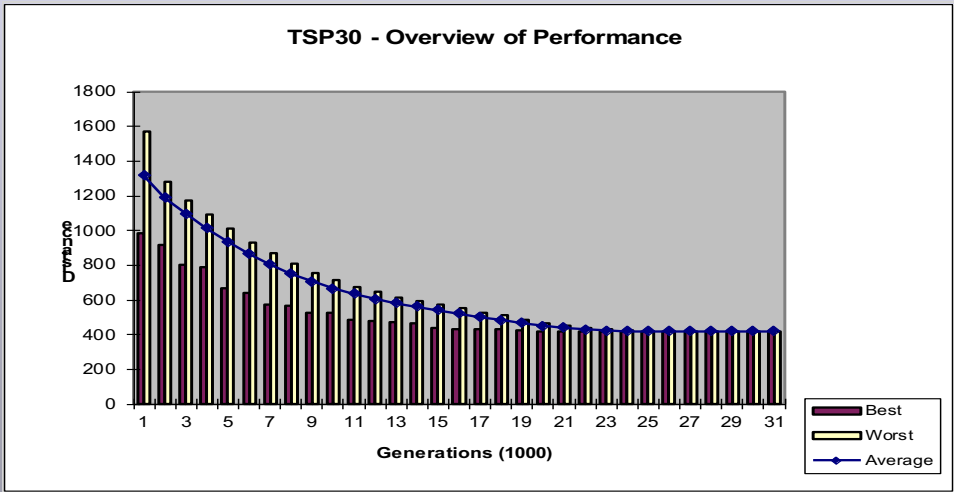
\includegraphics[scale=0.4]{images/lec04-pic47.png}
\end{figure}
\end{frame}

\end{document}
